
    % \subsection{Ackermann steering mode}
    % \label{subsec:ackermann_mode}
    
    % To model the Ackermann configuration, instead of using the full kinematic model of a four-wheeled Ackermann robot, a simplified approach is typically adopted by considering a two-wheeled model where both wheels are located along the central axis of the robot. This approximation is known as the bicycle kinematic model \cite{Sarcinelli-Filho2023_2}. It is known that the left and right wheels of a vehicle with Ackermann steering must rotate at different speeds during a turn, requiring different steering angles for each wheel. The mechanical structure of the Ackermann configuration addresses this difference in steering angles, making the bicycle kinematic model, illustrated in Figure \ref{fig:ackermann_mode}, a feasible approximation for such a vehicle.
    
    % \begin{figure}[!b]
    %     \centering
    %     \includegraphics[width=1\linewidth]{images/limo_bike.jpg}
    %     \caption{2D Kinematics of a car-like robot simplified as bicycle kinematic model. The rear axis position vector, $\bs{x}$, is translated by a distance $a$, resulting in a new position vector $\bs{x}_c$.}
    %     \label{fig:ackermann_mode}
    % \end{figure}
    
    % From such a figure, one gets the equation
    % \begin{equation}
    %     \begin{bmatrix} \dot{x}_c \\ \dot{y}_c \end{bmatrix}=\begin{bmatrix} c_\psi & -a s_\psi \\ s_\psi & a c_\psi \end{bmatrix}\begin{bmatrix} v \\ \omega \end{bmatrix},
    % \end{equation}
    % \noindent from which the same controller characterized in \eqref{eq:kinematic_controller_differential} and \eqref{eq:ff_fb_law} is obtained. Nonetheless, the high-level control signal for the Ackermann steering mode is $\bs u_a = \begin{bmatrix}v & \delta\end{bmatrix}^T$, in which $v$ is the linear velocity, already obtained in \eqref{eq:kinematic_controller_differential} and \eqref{eq:ff_fb_law}, and $\delta$ is the steering angle. To get $\delta$, one should consider the nonholonomic restriction applied to the front wheel, as illustrated in Figure~\ref{fig:ackermann_mode}, or
    % \begin{equation}
    %     L\omega \cos(\delta) - v\cos\left(\frac{\pi}{2}-\delta\right) = L\omega \cos(\delta) -v\sin(\delta) = 0,
    % \end{equation}
    % \noindent resulting in $\delta=\arctan{\left(\frac{L\omega}{v}\right)}$, where $L = 0.2~m$ is the distance between the rear and front wheels. This way the control signal $\bs u_a$ for the Ackermann mode of LIMO is obtained. The minimum rotation radius for the LIMO in Ackermann mode is $0.40~m$, corresponding to the maximum steering angle of $0.49~\ rad$ ($28^\circ)$.
    
    % Table \ref{tab:control_inputs} summarizes the control signals and their respective bounds for each driving mode of LIMO.
    % \begin{table}[h!]
    % \renewcommand{\arraystretch}{2}
    % \centering 
    % \caption{Control inputs and their respective limits.}
    % \label{tab:control_inputs}
    % \resizebox{1\columnwidth}{!}{ % Resize to half the column width
    % %\setlength{\extrarowheight}{2pt}            
    % \begin{tabular}{|c|c|}
    % \hline
    % \multirow{2}{*}{\textbf{Mode}} & \textbf{Control input}  \\ 
    % & \textbf{Limits} \\ \hline 
    % \multirow{2}{*}{Differential/Tracked} & $\bs{u} = \left[ v \quad \omega \right]^T$ \\ 
    % & $\bs{u} = \left[ \pm 1 \ m/s \quad \pm 3.14 \ rad/s \right]^T$  \\ 
    % \hline
    % \multirow{2}{*}{Omnidirectional} & $\bs{u}_o = \left[ \dot{x}^b \quad \dot{y}^b \quad \omega \right]^T$ \\ 
    % & $\bs{u}_o = \left[ \pm 1 \ m/s \quad \pm 1 \ m/s \quad \pm 3.14 \ rad/s \right]^T$ \\ 
    % \hline
    % \multirow{2}{*}{Ackermann} & $\bs{u}_a = \left[ v \quad \delta \right]^T $ \\ 
    % & $\bs{u}_a = \left[ \pm 1\ m/s \quad \pm 0.49\ rad \right]^T$  \\
    % \hline
    % \end{tabular}
    % }
    % \end{table}

\subsubsection{Modo de direção Ackermann}
    \label{subsec:ackermann_mode}
    
    Para modelar a configuração Ackermann, em vez de usar o modelo cinemático completo de um robô Ackermann de quatro rodas, uma abordagem simplificada é normalmente adotada, considerando um modelo de duas rodas onde ambas as rodas estão localizadas ao longo do eixo central do robô. Essa aproximação é conhecida como o modelo cinemático de bicicleta \cite{Sarcinelli-Filho2023_2}. É sabido que as rodas esquerda e direita de um veículo com direção Ackermann devem girar a velocidades diferentes durante uma curva, exigindo diferentes ângulos de direção para cada roda. A estrutura mecânica da configuração Ackermann aborda essa diferença nos ângulos de direção, tornando o modelo cinemático de bicicleta, ilustrado na Figura \ref{fig:ackermann_mode}, uma aproximação viável para tal veículo.
    
    \begin{figure}[htb]
        \centering
        \caption{Cinemática 2D de um robô semelhante a um carro simplificado como modelo cinemático de bicicleta.}
        \label{fig:ackermann_mode}
        \includegraphics[width=0.4\linewidth]{limo_bike.jpg}
        \sourceParbox[0.8\linewidth]
        \note[0.8\linewidth][O vetor de posição do eixo traseiro, $\bs{x}$, é traduzido por uma distância $a$, resultando em um novo vetor de posição $\bs{x}_c$.]
    \end{figure}
    
    A partir de tal figura, obtém-se a equação
    
    \begin{equation}
        \begin{bmatrix} \dot{x}_c \\ \dot{y}_c \end{bmatrix}=\begin{bmatrix} c_\psi & -a s_\psi \\ s_\psi & a c_\psi \end{bmatrix}\begin{bmatrix} v \\ \omega \end{bmatrix},
    \end{equation}
    
    \noindent da qual o mesmo controlador caracterizado na \eqref{eq:kinematic_controller_differential} e \eqref{eq:ff_fb_law} é obtido. No entanto, o sinal de controle de alto nível para o modo de direção Ackermann é $\bs u_a = \begin{bmatrix}v & \delta\end{bmatrix}^T$, em que $v$ é a velocidade linear, já obtida na \eqref{eq:kinematic_controller_differential} e \eqref{eq:ff_fb_law}, e $\delta$ é o ângulo de direção. Para obter $\delta$, deve-se considerar a restrição não holonômica aplicada à roda dianteira, conforme ilustrado na Figura~\ref{fig:ackermann_mode}, ou
    \begin{equation}
        L\omega \cos(\delta) - v\cos\left(\frac{\pi}{2}-\delta\right) = L\omega \cos(\delta) -v\sin(\delta) = 0,
    \end{equation}
    \noindent resultando em $\delta=\arctan{\left(\frac{L\omega}{v}\right)}$, onde $L = 0.2~m$ é a distância entre as rodas traseira e dianteira. Dessa forma, o sinal de controle $\bs u_a$ para o modo Ackermann do LIMO é obtido. O raio de rotação mínimo para o LIMO no modo Ackermann é de $0.40~m$, correspondente ao ângulo de direção máximo de $0.49~ rad$ ($28^\circ$).
    
    A Tabela \ref{tab:control_inputs} resume os sinais de controle e seus respectivos limites para cada modo de condução do LIMO.
    
    % \begin{table}[htb]
    %     \renewcommand{\arraystretch}{2}
    %     \centering 
    %     \caption{Entradas de controle e seus respectivos limites.}
    %     \label{tab:control_inputs}
    %     \resizebox{0.5\columnwidth}{!}{ % Redimensionar para metade da largura da coluna
    %         \begin{tabular}{|c|c|}
    %             \hline
    %             \multirow{2}{*}{\textbf{Modo}} & \textbf{Entrada de controle}  \\ 
    %             & \textbf{Limites} \\ \hline 
    %             \multirow{2}{*}{Diferencial/Com esteiras} & $\bs{u} = \left[ v \quad \omega \right]^T$ \\ 
    %             & $\bs{u} = \left[ \pm 1 \ m/s \quad \pm 3.14 \ rad/s \right]^T$  \\ 
    %             \hline
    %             \multirow{2}{*}{Omnidirecional} & $\bs{u}_o = \left[ \dot{x}^b \quad \dot{y}^b \quad \omega \right]^T$ \\ 
    %             & $\bs{u}_o = \left[ \pm 1 \ m/s \quad \pm 1 \ m/s \quad \pm 3.14 \ rad/s \right]^T$ \\ 
    %             \hline
    %             \multirow{2}{*}{Ackermann} & $\bs{u}_a = \left[ v \quad \delta \right]^T $ \\ 
    %             & $\bs{u}_a = \left[ \pm 1\ m/s \quad \pm 0.49\ rad \right]^T$  \\
    %             \hline
    %         \end{tabular}
    %     }
    % \end{table}

    \begin{table}[htb]
       \renewcommand{\arraystretch}{2}
        \centering 
        \caption{Entradas de controle e seus respectivos limites.}
        \label{tab:control_inputs}
        \resizebox{0.8\columnwidth}{!}{ % Redimensionar para metade da largura da coluna
            \begin{tabular}{|c|c|c|c|}
                \hline
                \textbf{Modo}                   &  Diferencial/Com esteiras    &    Omnidirecional    &    \textit{Ackermann}\\ \hline
                \textbf{Entrada de controle}    &    $\bs{u} = \left[ v \quad \omega \right]^T$    &  $\bs{u}_o = \left[ \dot{x}^b \quad \dot{y}^b \quad \omega \right]^T$  &  $\bs{u}_a = \left[ v \quad \delta \right]^T $  \\ \hline 
                \textbf{Limites} &  $\bs{u} = \left[ \pm 1 \ m/s \quad \pm 3.14 \ rad/s \right]^T$   &  $\bs{u}_o = \left[ \pm 1 \ m/s \quad \pm 1 \ m/s \quad \pm 3.14 \ rad/s \right]^T$  &  $\bs{u}_a = \left[ \pm 1\ m/s \quad \pm 0.49\ rad \right]^T$   \\ \hline
            \end{tabular}
        }
    \end{table}
